\documentclass[aspectratio=169]{beamer}

\usetheme{Madrid}
\usecolortheme{default}

\usepackage[utf8]{inputenc}
\usepackage[T1]{fontenc}
\usepackage{lmodern}
\usepackage{amsmath,amssymb}
\usepackage{booktabs}
\usepackage{array}
\usepackage{colortbl}
\usepackage{pifont}
\usepackage{listings}
\usepackage{tikz}
\usepackage{appendixnumberbeamer}
\usetikzlibrary{arrows.meta,positioning,shapes.geometric,fit,calc,backgrounds}

% --- Color Palette ---
\definecolor{spinNavy}{RGB}{24, 52, 92}
\definecolor{spinTeal}{RGB}{26, 115, 138}
\definecolor{spinGreen}{RGB}{36, 122, 74}
\definecolor{spinRed}{RGB}{184, 44, 44}
\definecolor{spinAmber}{RGB}{186, 114, 18}
\definecolor{spinLight}{RGB}{244, 247, 250}
\definecolor{spinGray}{RGB}{100, 112, 126}

% --- Beamer Styling ---
\setbeamercolor{structure}{fg=spinNavy}
\setbeamercolor{palette primary}{bg=spinNavy,fg=white}
\setbeamercolor{palette secondary}{bg=spinTeal!85!spinNavy,fg=white}
\setbeamercolor{palette tertiary}{bg=spinNavy!85!black,fg=white}
\setbeamercolor{palette quaternary}{bg=spinNavy,fg=white}
\setbeamercolor{titlelike}{parent=palette primary,bg=spinNavy,fg=white}
\setbeamercolor{frametitle}{bg=spinNavy,fg=white}
\setbeamercolor{block title}{bg=spinNavy,fg=white}
\setbeamercolor{block body}{bg=spinLight,fg=black}
\setbeamercolor{button}{bg=spinTeal,fg=white}

\setbeamertemplate{navigation symbols}{}
\setbeamertemplate{blocks}[rounded][shadow=false]
\setbeamertemplate{itemize items}[triangle]
\setbeamertemplate{itemize subitem}[circle]

% Check / cross helpers
\newcommand{\cmark}{\textcolor{spinGreen}{\ding{51}}}
\newcommand{\xmark}{\textcolor{spinRed}{\ding{55}}}

% Ragged-right table column helper
\newcolumntype{L}[1]{>{\raggedright\arraybackslash}p{#1}}

% --- PROMELA Listings Style ---
\lstdefinelanguage{PROMELA}{
  morekeywords={proctype,active,init,run,chan,mtype,byte,bit,atomic,if,fi,do,od,else,break,assert,of},
  sensitive=true,
  morecomment=[s]{/*}{*/},
  morestring=[b]"
}
\lstset{
  language=PROMELA,
  basicstyle=\ttfamily\scriptsize,
  columns=fullflexible,
  keepspaces=true,
  keywordstyle=\color{spinNavy}\bfseries,
  commentstyle=\color{spinGray}\itshape,
  stringstyle=\color{spinTeal},
  showstringspaces=false,
  breaklines=false,
  frame=single,
  rulecolor=\color{spinNavy!25},
  backgroundcolor=\color{spinLight},
  aboveskip=2pt,
  belowskip=2pt,
  xleftmargin=4pt,
  xrightmargin=4pt
}

% --- Metadata ---
\title[The Model Checker SPIN]{The Model Checker SPIN}
\subtitle{Gerard J. Holzmann, IEEE TSE 23(5), 1997 --- Paper Presentation}
\author{Ming}
\institute{Formal Methods in Software Development}
\date{\today}

\begin{document}

% ==============================================================================
% Frame 1: Title (~0.5 min)
% ==============================================================================
\begin{frame}
  \titlepage
  \note{0.5 min: Introduce Holzmann (IEEE TSE 23(5), pp. 279--295, May 1997) and the focus of the talk.}
\end{frame}

% ==============================================================================
% Frame 2: Presentation Roadmap (~0.5 min)
% ==============================================================================
\begin{frame}{Presentation Roadmap}
  \begin{itemize}
    \item \textbf{Objective:} Explain model checking in general, how SPIN and PROMELA fit in, target application domains, and walk through one full case study (\textbf{30 min total, incl.\ Q\&A}).
    \item \textbf{Scope:} Focus on \textbf{core concepts, visual intuition, and case study}; internal search and memory optimizations are omitted to fit the 30-minute budget.
  \end{itemize}
  \vspace{0.5em}
  \begin{center}
    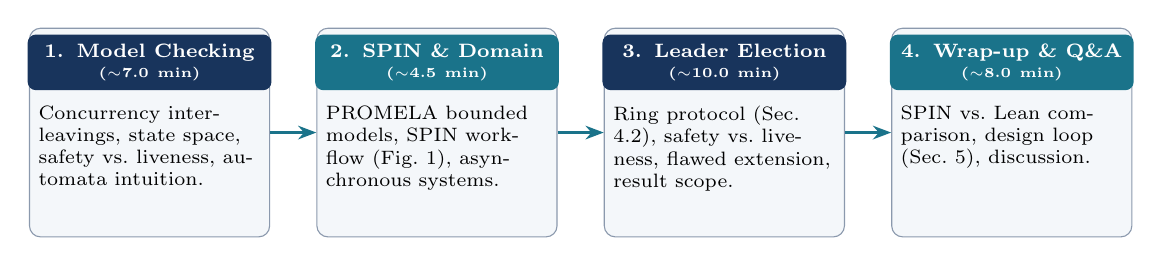
\begin{tikzpicture}[
      card/.style={draw=spinNavy!50, fill=spinLight, rounded corners=4pt,
                   text width=3.05cm, minimum height=2.65cm, inner sep=0pt},
      hdr/.style={fill=spinNavy, text=white, rounded corners=3pt, font=\scriptsize\bfseries,
                  text width=2.85cm, align=center, inner sep=3.5pt},
      bdy/.style={text width=2.82cm, align=left, font=\scriptsize, inner sep=2pt},
      arr/.style={->, >=Stealth, thick, color=spinTeal}
    ]
      \node[card] (c1) at (0,0) {};
      \node[hdr, anchor=north] (h1) at ($(c1.north)+(0,-0.08)$) {1. Model Checking\\[-1pt]{\tiny ($\sim$7.0 min)}};
      \node[bdy, anchor=north] at ($(h1.south)+(0,-0.12)$)
        {Concurrency interleavings, state space, safety vs.\ liveness, automata intuition.};

      \node[card] (c2) at (3.65,0) {};
      \node[hdr, fill=spinTeal, anchor=north] (h2) at ($(c2.north)+(0,-0.08)$) {2. SPIN \& Domain\\[-1pt]{\tiny ($\sim$4.5 min)}};
      \node[bdy, anchor=north] at ($(h2.south)+(0,-0.12)$)
        {PROMELA bounded models, SPIN workflow (Fig.\ 1), asynchronous systems.};

      \node[card] (c3) at (7.30,0) {};
      \node[hdr, anchor=north] (h3) at ($(c3.north)+(0,-0.08)$) {3. Leader Election\\[-1pt]{\tiny ($\sim$10.0 min)}};
      \node[bdy, anchor=north] at ($(h3.south)+(0,-0.12)$)
        {Ring protocol (Sec.\ 4.2), safety vs.\ liveness, flawed extension, result scope.};

      \node[card] (c4) at (10.95,0) {};
      \node[hdr, fill=spinTeal, anchor=north] (h4) at ($(c4.north)+(0,-0.08)$) {4. Wrap-up \& Q\&A\\[-1pt]{\tiny ($\sim$8.0 min)}};
      \node[bdy, anchor=north] at ($(h4.south)+(0,-0.12)$)
        {SPIN vs.\ Lean comparison, design loop (Sec.\ 5), discussion.};

      \draw[arr] (c1.east) -- (c2.west);
      \draw[arr] (c2.east) -- (c3.west);
      \draw[arr] (c3.east) -- (c4.west);
    \end{tikzpicture}
  \end{center}
  \note{0.5 min: Preview the 4 parts (~25.5 min talk + ~4.5 min Q&A).}
\end{frame}

% ==============================================================================
\section{What Is Model Checking?}
% ==============================================================================

% Frame 3 (~2.0 min)
\begin{frame}{Why Concurrent Software Is Hard to Verify}
  \begin{itemize}
    \item Two concurrent processes $A$ and $B$ each increment a shared variable $x$ (initially $x = 0$):
      \quad $A:\; A_1:\, a = x;\; A_2:\, x = a + 1$ \qquad
      $B:\; B_1:\, b = x;\; B_2:\, x = b + 1$
    \item Individually both look trivial, yet \textbf{interleaving order} changes the final value of $x$.
    \item \textbf{Why testing falls short:} Running tests exercises only a few schedules; subtle bugs hide in rare interleavings.
  \end{itemize}
  \vspace{0.3em}
  \begin{center}
    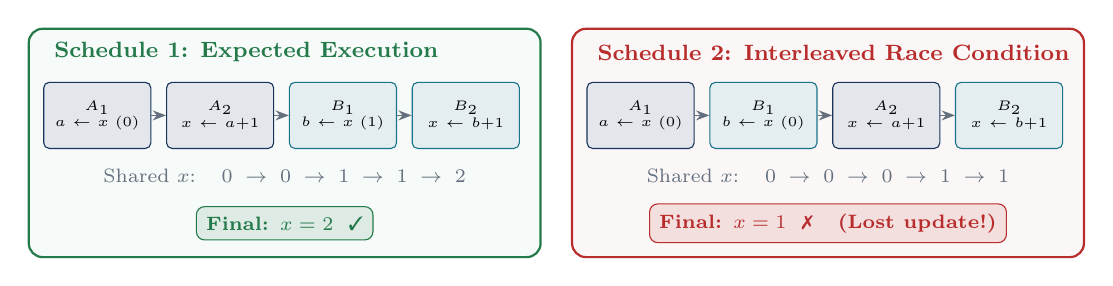
\begin{tikzpicture}[
      stepA/.style={draw=spinNavy, fill=spinNavy!12, rounded corners=2pt,
                    text width=1.22cm, minimum height=0.84cm, align=center, font=\tiny, inner sep=2pt},
      stepB/.style={draw=spinTeal, fill=spinTeal!12, rounded corners=2pt,
                    text width=1.22cm, minimum height=0.84cm, align=center, font=\tiny, inner sep=2pt},
      arr/.style={->, >=Stealth, thin, color=spinGray}
    ]
      % Left card: Schedule 1
      \draw[draw=spinGreen, thick, fill=spinGreen!4, rounded corners=5pt] (-0.25,-1.35) rectangle (6.25,1.55);
      \node[font=\footnotesize\bfseries, text=spinGreen, anchor=west] at (-0.05,1.25) {Schedule 1: Expected Execution};
      \node[stepA] (s11) at (0.62,0.45) {\textbf{$A_1$}\\$a \leftarrow x$ ($0$)};
      \node[stepA] (s12) at (2.18,0.45) {\textbf{$A_2$}\\$x \leftarrow a{+}1$};
      \node[stepB] (s13) at (3.74,0.45) {\textbf{$B_1$}\\$b \leftarrow x$ ($1$)};
      \node[stepB] (s14) at (5.30,0.45) {\textbf{$B_2$}\\$x \leftarrow b{+}1$};
      \draw[arr] (s11) -- (s12); \draw[arr] (s12) -- (s13); \draw[arr] (s13) -- (s14);
      \node[font=\scriptsize, text=spinGray] at (3.00,-0.32) {Shared $x$: \; $0 \;\to\; 0 \;\to\; 1 \;\to\; 1 \;\to\; 2$};
      \node[draw=spinGreen, fill=spinGreen!15, rounded corners=3pt, font=\scriptsize\bfseries, text=spinGreen, inner sep=3.5pt]
        at (3.00,-0.92) {Final: $x = 2$ \;\cmark};

      % Right card: Schedule 2
      \draw[draw=spinRed, thick, fill=spinRed!4, rounded corners=5pt] (6.65,-1.35) rectangle (13.15,1.55);
      \node[font=\footnotesize\bfseries, text=spinRed, anchor=west] at (6.85,1.25) {Schedule 2: Interleaved Race Condition};
      \node[stepA] (s21) at (7.52,0.45) {\textbf{$A_1$}\\$a \leftarrow x$ ($0$)};
      \node[stepB] (s22) at (9.08,0.45) {\textbf{$B_1$}\\$b \leftarrow x$ ($0$)};
      \node[stepA] (s23) at (10.64,0.45) {\textbf{$A_2$}\\$x \leftarrow a{+}1$};
      \node[stepB] (s24) at (12.20,0.45) {\textbf{$B_2$}\\$x \leftarrow b{+}1$};
      \draw[arr] (s21) -- (s22); \draw[arr] (s22) -- (s23); \draw[arr] (s23) -- (s24);
      \node[font=\scriptsize, text=spinGray] at (9.90,-0.32) {Shared $x$: \; $0 \;\to\; 0 \;\to\; 0 \;\to\; 1 \;\to\; 1$};
      \node[draw=spinRed, fill=spinRed!15, rounded corners=3pt, font=\scriptsize\bfseries, text=spinRed, inner sep=3.5pt]
        at (9.90,-0.92) {Final: $x = 1$ \;\xmark\quad (Lost update!)};
    \end{tikzpicture}
  \end{center}
  \note{2.0 min: Walk through the two schedules and motivate exhaustive checking.}
\end{frame}

% Frame 4 (~2.5 min)
\begin{frame}{States, Transitions, and Counterexamples}
  \begin{itemize}
    \item A \textbf{state} captures both data and control points: $(x, a, b;\; \text{pc}_A, \text{pc}_B)$, with atomic steps as \textbf{transitions}.
    \item Distinct execution paths can \textbf{merge} at the same state (e.g., $A_1{\to}B_1$ and $B_1{\to}A_1$ both reach $(0,0,0;\;1,1)$).
    \item \textbf{Property:} ``When both terminate, $x = 2$.'' A single reachable violating path is a \textbf{counterexample}.
  \end{itemize}
  \vspace{0.2em}
  \begin{center}
    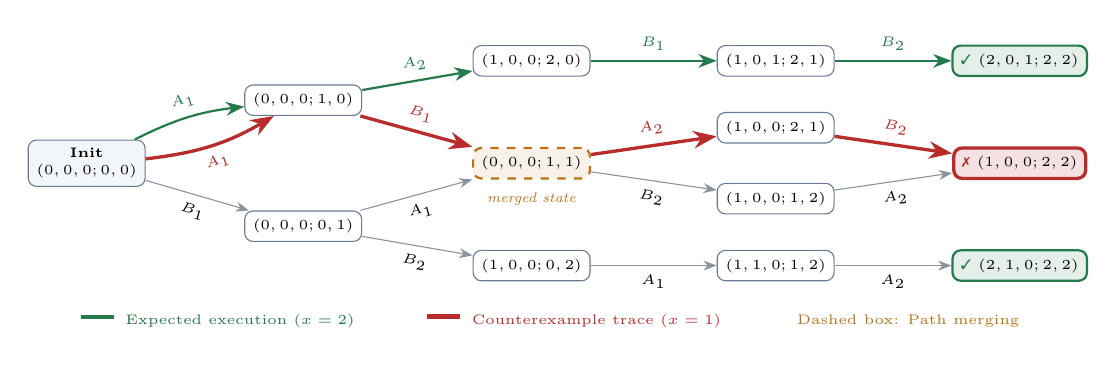
\begin{tikzpicture}[
      st/.style={draw=spinNavy!65, fill=white, rounded corners=3pt, font=\tiny, inner sep=3pt, align=center},
      merged/.style={draw=spinAmber, thick, dashed, fill=spinAmber!10, rounded corners=3pt, font=\tiny, inner sep=3pt, align=center},
      ok/.style={draw=spinGreen, thick, fill=spinGreen!12, rounded corners=3pt, font=\tiny\bfseries, inner sep=3pt, align=center},
      err/.style={draw=spinRed, very thick, fill=spinRed!14, rounded corners=3pt, font=\tiny\bfseries, inner sep=3pt, align=center},
      edge/.style={->, >=Stealth, draw=spinGray!75, font=\tiny},
      okedge/.style={->, >=Stealth, thick, draw=spinGreen, font=\tiny},
      erredge/.style={->, >=Stealth, very thick, draw=spinRed, font=\tiny}
    ]
      % Column 0
      \node[st, fill=spinLight] (S0) at (0,1.45) {\textbf{Init}\\$(0,0,0;0,0)$};
      % Column 1
      \node[st] (S1) at (2.75,2.25) {$(0,0,0;1,0)$};
      \node[st] (S2) at (2.75,0.65) {$(0,0,0;0,1)$};
      % Column 2
      \node[st] (S3) at (5.65,2.75) {$(1,0,0;2,0)$};
      \node[merged] (S4) at (5.65,1.45) {$(0,0,0;1,1)$};
      \node[font=\tiny\itshape, text=spinAmber] at (5.65,1.00) {merged state};
      \node[st] (S5) at (5.65,0.15) {$(1,0,0;0,2)$};
      % Column 3
      \node[st] (S6) at (8.75,2.75) {$(1,0,1;2,1)$};
      \node[st] (S7) at (8.75,1.90) {$(1,0,0;2,1)$};
      \node[st] (S8) at (8.75,1.00) {$(1,0,0;1,2)$};
      \node[st] (S9) at (8.75,0.15) {$(1,1,0;1,2)$};
      % Column 4
      \node[ok]  (G1) at (11.85,2.75) {\cmark\ $(2,0,1;2,2)$};
      \node[err] (F)  at (11.85,1.45) {\xmark\ $(1,0,0;2,2)$};
      \node[ok]  (G2) at (11.85,0.15) {\cmark\ $(2,1,0;2,2)$};

      % Normal green path
      \draw[okedge] (S0) to[bend left=10] node[above, sloped, text=spinGreen] {$A_1$} (S1);
      \draw[okedge] (S1) -- node[above, sloped, text=spinGreen] {$A_2$} (S3);
      \draw[okedge] (S3) -- node[above, text=spinGreen] {$B_1$} (S6);
      \draw[okedge] (S6) -- node[above, text=spinGreen] {$B_2$} (G1);

      % Counterexample red path
      \draw[erredge] (S0) to[bend right=12] node[below, sloped, text=spinRed] {$A_1$} (S1);
      \draw[erredge] (S1) -- node[above, sloped, text=spinRed] {$B_1$} (S4);
      \draw[erredge] (S4) -- node[above, sloped, text=spinRed] {$A_2$} (S7);
      \draw[erredge] (S7) -- node[above, sloped, text=spinRed] {$B_2$} (F);

      % Other valid transitions
      \draw[edge] (S0) -- node[below, sloped] {$B_1$} (S2);
      \draw[edge] (S2) -- node[below, sloped] {$A_1$} (S4);
      \draw[edge] (S2) -- node[below, sloped] {$B_2$} (S5);
      \draw[edge] (S4) -- node[below, sloped] {$B_2$} (S8);
      \draw[edge] (S8) -- node[below, sloped] {$A_2$} (F);
      \draw[edge] (S5) -- node[below] {$A_1$} (S9);
      \draw[edge] (S9) -- node[below] {$A_2$} (G2);

      % Legend
      \node[font=\tiny, text=spinGreen, anchor=west] at (-0.2,-0.55) {\rule[2pt]{12pt}{1.2pt}\; Expected execution ($x=2$)};
      \node[font=\tiny, text=spinRed, anchor=west]   at (4.2,-0.55) {\rule[2pt]{12pt}{1.6pt}\; Counterexample trace ($x=1$)};
      \node[font=\tiny, text=spinAmber, anchor=west] at (8.9,-0.55) {Dashed box: Path merging};
    \end{tikzpicture}
  \end{center}
  \note{2.5 min: Show state tuple, merged node (0,0,0;1,1), and red counterexample trace.}
\end{frame}

% Frame 5 (~2.5 min)
\begin{frame}{Automata-Based Model Checking: Intuition (Sec.\ 2)}
  \begin{itemize}
    \item \textbf{System model ($S$):} Each process template maps to a finite automaton; global behavior is their asynchronous interleaving product.
    \item \textbf{Properties in LTL:} \textbf{Safety} (``nothing bad ever happens'' --- finite bad prefix) vs.\ \textbf{Liveness} (``something good eventually happens'' --- cyclic/infinite violation).
    \item \textbf{Vardi--Wolper check:} Negate claim ($\neg\varphi \to$ B\"uchi automaton $B_{\neg\varphi}$) and test language emptiness: $L(S) \cap L(B_{\neg\varphi}) = \emptyset$.
  \end{itemize}
  \vspace{0.3em}
  \begin{center}
    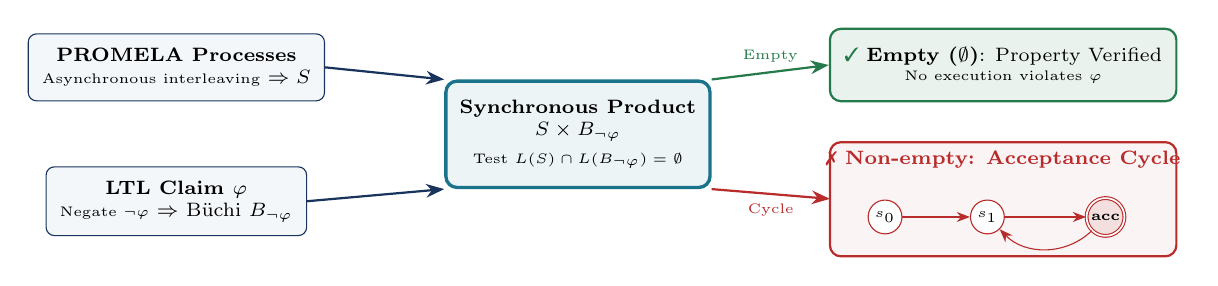
\begin{tikzpicture}[
      box/.style={draw=spinNavy, fill=spinLight, rounded corners=3pt, font=\scriptsize,
                  minimum height=0.85cm, align=center, inner sep=5pt},
      prod/.style={draw=spinTeal, very thick, fill=spinTeal!8, rounded corners=4pt, font=\scriptsize,
                   minimum width=3.1cm, minimum height=1.35cm, align=center, inner sep=5pt},
      arr/.style={->, >=Stealth, thick, color=spinNavy}
    ]
      % Left inputs
      \node[box, minimum width=2.9cm] (proc) at (0,0.85) {\textbf{PROMELA Processes}\\{\tiny Asynchronous interleaving} $\Rightarrow S$};
      \node[box, minimum width=2.9cm] (ltl)  at (0,-0.85) {\textbf{LTL Claim $\varphi$}\\{\tiny Negate $\neg\varphi$} $\Rightarrow$ B\"uchi $B_{\neg\varphi}$};

      % Center product
      \node[prod] (prod) at (5.1,0) {\textbf{Synchronous Product}\\$S \times B_{\neg\varphi}$\\[2pt]{\tiny Test $L(S) \cap L(B_{\neg\varphi}) = \emptyset$}};
      \draw[arr] (proc.east) -- (prod.north west);
      \draw[arr] (ltl.east)  -- (prod.south west);

      % Right Top: Verified
      \node[draw=spinGreen, thick, fill=spinGreen!10, rounded corners=4pt, font=\scriptsize,
            minimum width=4.4cm, minimum height=0.92cm, align=center] (ok) at (10.5,0.88)
        {\cmark\ \textbf{Empty ($\emptyset$)}: Property Verified\\[-1pt]{\tiny No execution violates $\varphi$}};
      \draw[->, >=Stealth, thick, color=spinGreen] (prod.north east) -- node[above, font=\tiny, text=spinGreen] {Empty} (ok.west);

      % Right Bottom: Counterexample lasso
      \draw[draw=spinRed, thick, fill=spinRed!5, rounded corners=4pt] (8.3,-1.55) rectangle (12.7,-0.10);
      \node[font=\scriptsize\bfseries, text=spinRed] at (10.5,-0.32) {\xmark\ Non-empty: Acceptance Cycle};
      \node[circle, draw=spinRed, fill=white, inner sep=1.5pt, font=\tiny] (q0) at (9.0,-1.05) {$s_0$};
      \node[circle, draw=spinRed, fill=white, inner sep=1.5pt, font=\tiny] (q1) at (10.3,-1.05) {$s_1$};
      \node[circle, draw=spinRed, double, fill=spinRed!15, inner sep=1.2pt, font=\tiny\bfseries] (q2) at (11.8,-1.05) {acc};
      \draw[->, >=Stealth, color=spinRed] (q0) -- (q1);
      \draw[->, >=Stealth, color=spinRed] (q1) -- (q2);
      \draw[->, >=Stealth, color=spinRed] (q2) to[bend left=45] (q1);
      \draw[->, >=Stealth, thick, color=spinRed] (prod.south east) -- node[below, font=\tiny, text=spinRed] {Cycle} (8.3,-0.82);
    \end{tikzpicture}
  \end{center}
  \note{2.5 min: Explain why negation turns safety/liveness checking into searching for an empty product or acceptance cycle.}
\end{frame}

% ==============================================================================
\section{SPIN, PROMELA, and Application Domain}
% ==============================================================================

% Frame 6 (~2.5 min)
\begin{frame}{How SPIN \& PROMELA Fit Together (Sec.\ 1.1, Fig.\ 1)}
  \begin{columns}[T]
    \begin{column}{0.48\textwidth}
      \textbf{\textcolor{spinNavy}{PROMELA (Modeling Language)}}
      \begin{itemize}
        \item Process templates (\texttt{proctype}), rendezvous, buffered channels (\texttt{chan}), shared variables.
        \item Strictly \textbf{bounded} (finite states, ranges, buffer capacities) $\Rightarrow$ decidable!
      \end{itemize}
    \end{column}
    \begin{column}{0.48\textwidth}
      \textbf{\textcolor{spinTeal}{SPIN (Verification Tool)}}
      \begin{itemize}
        \item Parses PROMELA + LTL claims (via XSPIN front-end).
        \item Runs \textbf{interactive simulation}, generates an \textbf{on-the-fly C verifier}, and replays counterexamples.
      \end{itemize}
    \end{column}
  \end{columns}
  \vspace{0.4em}
  \begin{center}
    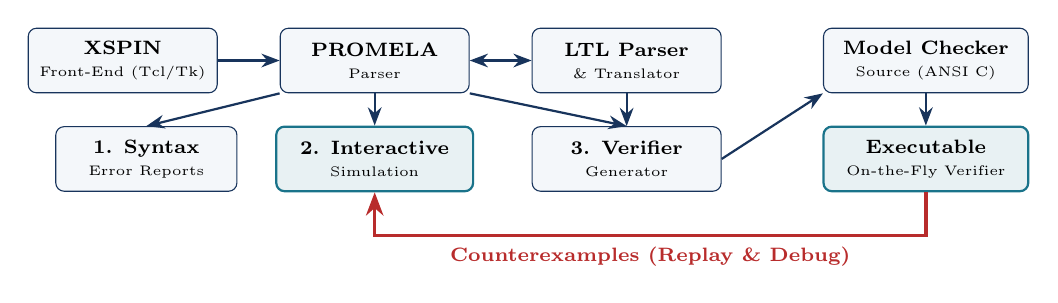
\begin{tikzpicture}[
      bx/.style={draw=spinNavy, fill=spinLight, rounded corners=3pt, font=\scriptsize,
                 align=center, minimum height=0.82cm, inner sep=4pt},
      hi/.style={draw=spinTeal, thick, fill=spinTeal!10, rounded corners=3pt, font=\scriptsize,
                 align=center, minimum height=0.82cm, inner sep=4pt},
      arr/.style={->, >=Stealth, thick, color=spinNavy}
    ]
      % Top row
      \node[bx, minimum width=2.4cm] (xspin) at (0,1.25) {\textbf{XSPIN}\\{\tiny Front-End (Tcl/Tk)}};
      \node[bx, minimum width=2.4cm] (parse) at (3.2,1.25) {\textbf{PROMELA}\\{\tiny Parser}};
      \node[bx, minimum width=2.4cm] (ltl)   at (6.4,1.25) {\textbf{LTL Parser}\\{\tiny \& Translator}};

      \draw[arr] (xspin) -- (parse);
      \draw[<->, >=Stealth, thick, color=spinNavy] (parse) -- (ltl);

      % Middle branches
      \node[bx, minimum width=2.3cm] (syn) at (0.3,0.0) {\textbf{1. Syntax}\\{\tiny Error Reports}};
      \node[hi, minimum width=2.5cm] (sim) at (3.2,0.0) {\textbf{2. Interactive}\\{\tiny Simulation}};
      \node[bx, minimum width=2.4cm] (gen) at (6.4,0.0) {\textbf{3. Verifier}\\{\tiny Generator}};

      \draw[arr] (parse.south west) -- (syn.north);
      \draw[arr] (parse.south)      -- (sim.north);
      \draw[arr] (parse.south east) -- (gen.north);
      \draw[arr] (ltl.south)        -- (gen.north);

      % Right verifier chain
      \node[bx, minimum width=2.6cm] (csrc) at (10.2,1.25) {\textbf{Model Checker}\\{\tiny Source (ANSI C)}};
      \node[hi, minimum width=2.6cm] (exe)  at (10.2,0.0) {\textbf{Executable}\\{\tiny On-the-Fly Verifier}};

      \draw[arr] (gen.east) -- (csrc.south west);
      \draw[arr] (csrc) -- (exe);

      % Red counterexample feedback loop
      \draw[->, >=Stealth, very thick, color=spinRed]
        (exe.south) -- ++(0,-0.55) -| node[pos=0.25, below, font=\scriptsize\bfseries, text=spinRed]
        {Counterexamples (Replay \& Debug)} (sim.south);
    \end{tikzpicture}
  \end{center}
  \note{2.5 min: Walk through Paper Fig. 1 cleanly without mentioning optimization options.}
\end{frame}

% Frame 7 (~2.0 min)
\begin{frame}{Target Application Domain (Sec.\ 1, 2.2, 4.4)}
  \begin{itemize}
    \item \textbf{Core focus:} \textbf{Asynchronous software systems} and \textbf{process interactions} (abstracting away internal sequential computation)---contrasting with synchronous hardware checkers.
  \end{itemize}
  \vspace{0.35em}
  \begin{center}
    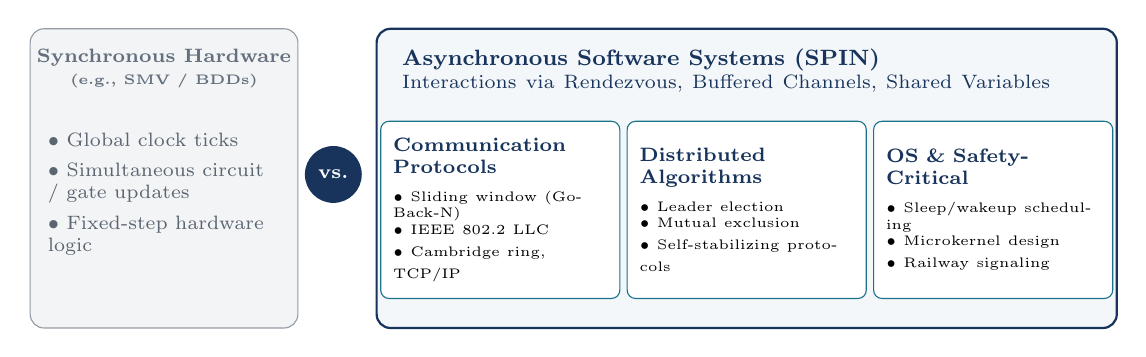
\begin{tikzpicture}[
      cluster/.style={draw=spinTeal, fill=white, rounded corners=3pt,
                      text width=2.72cm, minimum height=2.25cm, align=left, inner sep=4.5pt, font=\scriptsize}
    ]
      % Left: Hardware contrast
      \draw[draw=spinGray!70, fill=spinGray!8, rounded corners=5pt] (-0.15,-1.95) rectangle (3.25,1.85);
      \node[font=\scriptsize\bfseries, text=spinGray, align=center] at (1.55,1.35) {Synchronous Hardware\\{\tiny (e.g., SMV / BDDs)}};
      \node[text width=2.95cm, font=\scriptsize, align=left, text=spinGray!90!black] at (1.55,-0.25) {
        $\bullet$ Global clock ticks\\[3pt]
        $\bullet$ Simultaneous circuit / gate updates\\[3pt]
        $\bullet$ Fixed-step hardware logic
      };

      % VS badge
      \node[circle, fill=spinNavy, text=white, font=\scriptsize\bfseries, inner sep=3.5pt] (vs) at (3.70,0.0) {vs.};

      % Right: SPIN Asynchronous Software + 3 domain clusters
      \draw[draw=spinNavy, thick, fill=spinLight, rounded corners=5pt] (4.25,-1.95) rectangle (13.65,1.85);
      \node[font=\footnotesize\bfseries, text=spinNavy, text width=8.9cm, align=left, anchor=north west] at (4.45,1.72)
        {Asynchronous Software Systems (SPIN)\\[-1pt]{\normalfont\scriptsize Interactions via Rendezvous, Buffered Channels, Shared Variables}};

      \node[cluster] (d1) at (5.82,-0.45) {%
        \textcolor{spinNavy}{\textbf{Communication\\Protocols}}\\[4pt]
        {\tiny $\bullet$ Sliding window (Go-Back-N)\\
        $\bullet$ IEEE 802.2 LLC\\
        $\bullet$ Cambridge ring, TCP/IP}
      };
      \node[cluster] (d2) at (8.95,-0.45) {%
        \textcolor{spinNavy}{\textbf{Distributed\\Algorithms}}\\[4pt]
        {\tiny $\bullet$ Leader election\\
        $\bullet$ Mutual exclusion\\
        $\bullet$ Self-stabilizing protocols}
      };
      \node[cluster] (d3) at (12.08,-0.45) {%
        \textcolor{spinNavy}{\textbf{OS \& Safety-\\Critical}}\\[4pt]
        {\tiny $\bullet$ Sleep/wakeup scheduling\\
        $\bullet$ Microkernel design\\
        $\bullet$ Railway signaling}
      };
    \end{tikzpicture}
  \end{center}
  \note{2.0 min: Answer what domain SPIN targets using Sec. 1, 2.2, and 4.4.}
\end{frame}

% ==============================================================================
\section{Case Study: Leader Election in a Ring}
% ==============================================================================

% Frame 8 (~2.5 min)
\begin{frame}{Problem \& Algorithm: Unidirectional Ring (Sec.\ 4.2)}
  \begin{columns}[T]
    \begin{column}{0.49\textwidth}
      \begin{itemize}
        \item Based on \textbf{Dolev, Klawe, and Rodeh (1982)} (via Raynal 1992).
        \item $N$ processes with unique IDs on a \textbf{unidirectional ring} linked by asynchronous FIFO channels.
        \item \textbf{Elimination rule:} Each \texttt{Active} node compares 3 consecutive IDs (\texttt{maximum}, \texttt{neighbourR}, \texttt{nr}).
        \item Only local maxima (\texttt{neighbourR > maximum \&\& neighbourR > nr}) stay \texttt{Active}; others become passive relays until the global max loops around.
      \end{itemize}
    \end{column}
    \begin{column}{0.48\textwidth}
      \begin{center}
        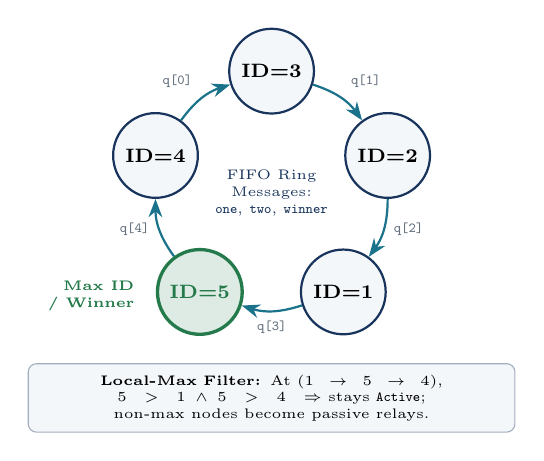
\begin{tikzpicture}[
          nd/.style={circle, draw=spinNavy, thick, fill=spinLight, minimum size=0.82cm,
                     font=\scriptsize\bfseries, align=center},
          win/.style={circle, draw=spinGreen, very thick, fill=spinGreen!15, minimum size=0.88cm,
                      font=\scriptsize\bfseries, text=spinGreen, align=center},
          chan/.style={->, >=Stealth, thick, color=spinTeal}
        ]
          % Appendix B exact N=5, I=3 ring order: ID=3 -> ID=2 -> ID=1 -> ID=5 -> ID=4 -> ID=3
          \node[nd]  (n1) at (90:1.55)   {ID=3};
          \node[nd]  (n2) at (18:1.55)   {ID=2};
          \node[nd]  (n3) at (-54:1.55)  {ID=1};
          \node[win] (n4) at (-126:1.55) {ID=5};
          \node[nd]  (n5) at (162:1.55)  {ID=4};

          \node[font=\tiny\bfseries, text=spinGreen, align=right, anchor=east] at ($(n4.west)+(-0.15,-0.05)$) {Max ID\\/ Winner};

          \draw[chan] (n1) to[bend left=18] node[above right, font=\tiny, text=spinGray] {\texttt{q[1]}} (n2);
          \draw[chan] (n2) to[bend left=18] node[right, font=\tiny, text=spinGray] {\texttt{q[2]}} (n3);
          \draw[chan] (n3) to[bend left=18] node[below, font=\tiny, text=spinGray] {\texttt{q[3]}} (n4);
          \draw[chan] (n4) to[bend left=18] node[left, font=\tiny, text=spinGray] {\texttt{q[4]}} (n5);
          \draw[chan] (n5) to[bend left=18] node[above left, font=\tiny, text=spinGray] {\texttt{q[0]}} (n1);

          \node[font=\tiny, text=spinNavy, align=center] at (0,0) {FIFO Ring\\Messages:\\\texttt{one}, \texttt{two}, \texttt{winner}};

          % Rule callout box underneath
          \node[draw=spinNavy!40, fill=spinLight, rounded corners=3pt, text width=5.9cm,
                font=\tiny, align=center, inner sep=4pt] at (0,-2.60)
            {\textbf{Local-Max Filter:} At $(1 \to 5 \to 4)$, $5 > 1 \land 5 > 4 \Rightarrow$ stays \texttt{Active};\\ non-max nodes become passive relays.};
        \end{tikzpicture}
      \end{center}
    \end{column}
  \end{columns}
  \note{2.5 min: Walk through Appendix B's exact 5-node ID layout and local-maximum elimination.}
\end{frame}

% Frame 9 (~2.5 min)
\begin{frame}[fragile]{Modeling Choices \& Distilled PROMELA (Appendix B)}
  \begin{columns}[T]
    \begin{column}{0.54\textwidth}
\begin{lstlisting}
#define N 5
#define L 10
mtype = {one, two, winner};
chan q[N] = [L] of {mtype, byte};
byte nr_leaders = 0;

proctype node(chan in, out; byte mynum)
{ ...
  :: in?one(nr) -> ... out!winner, nr;
  :: in?winner, nr ->
     if :: nr == mynum ->
           nr_leaders++;
           assert(nr_leaders == 1)
     fi
}
\end{lstlisting}
    \end{column}
    \begin{column}{0.43\textwidth}
      \begin{block}{Key Modeling Choices \& Assumptions}
        \begin{itemize}
          \item \textbf{Bounded model:} $N = 5$ processes, buffer capacity $L = 10 \ge 2N$.
          \item \textbf{Channels:} Reliable, lossless asynchronous FIFO message passing.
          \item \textbf{Initial state:} All $N$ nodes start \texttt{Active} with distinct IDs ($1\dots N$).
          \item \textbf{Instrumentation:} Global ghost counter \texttt{nr\_leaders} tracks elected leaders.
        \end{itemize}
      \end{block}
    \end{column}
  \end{columns}
  \note{2.5 min: Connect Appendix B PROMELA syntax directly to boundedness and modeling assumptions.}
\end{frame}

% Frame 10 (~3.0 min)
\begin{frame}{Properties Verified \& Catching a Flawed Extension}
  \begin{itemize}
    \item \textbf{Baseline ($N = 5$, Sec.\ 4.2):} Safety \texttt{[] (nr\_leaders <= 1)} vs.\ Liveness \texttt{<>[] (nr\_leaders == 1)} --- safety alone is vacuous if \emph{no} leader is ever elected!
    \item \textbf{Textbook Modification (Deferred Participation, Sec.\ 4.1.1, pp.\ 8--9):} Allowing nodes to join only on receiving the first message lets SPIN refute \texttt{assert(nr == N)}!
  \end{itemize}
  \vspace{0.35em}
  \begin{center}
    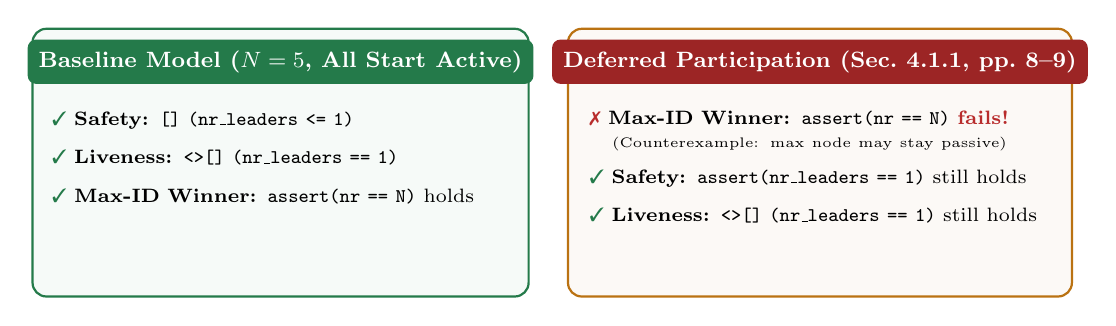
\begin{tikzpicture}
      % Left card: Baseline
      \draw[draw=spinGreen, thick, fill=spinGreen!4, rounded corners=5pt] (-0.1,-1.75) rectangle (6.2,1.65);
      \node[fill=spinGreen, text=white, rounded corners=3pt, font=\footnotesize\bfseries,
            minimum width=5.9cm, inner sep=4pt, anchor=north] (bh) at (3.05,1.52) {Baseline Model ($N = 5$, All Start Active)};
      \node[text width=5.8cm, font=\scriptsize, align=left, anchor=north] at ($(bh.south)+(0,-0.22)$) {
        \cmark\ \textbf{Safety:} \texttt{[] (nr\_leaders <= 1)}\\[6pt]
        \cmark\ \textbf{Liveness:} \texttt{<>[] (nr\_leaders == 1)}\\[6pt]
        \cmark\ \textbf{Max-ID Winner:} \texttt{assert(nr == N)} holds
      };

      % Right card: Deferred Participation
      \draw[draw=spinAmber, thick, fill=spinAmber!4, rounded corners=5pt] (6.7,-1.75) rectangle (13.1,1.65);
      \node[fill=spinRed!85!black, text=white, rounded corners=3pt, font=\footnotesize\bfseries,
            minimum width=5.95cm, inner sep=4pt, anchor=north] (dh) at (9.9,1.52) {Deferred Participation (Sec.\ 4.1.1, pp.\ 8--9)};
      \node[text width=5.85cm, font=\scriptsize, align=left, anchor=north] at ($(dh.south)+(0,-0.22)$) {
        \xmark\ \textbf{Max-ID Winner:} \texttt{assert(nr == N)} \textcolor{spinRed}{\textbf{fails!}}\\
        {\tiny\hspace{1.2em}(Counterexample: max node may stay passive)}\\[5pt]
        \cmark\ \textbf{Safety:} \texttt{assert(nr\_leaders == 1)} still holds\\[6pt]
        \cmark\ \textbf{Liveness:} \texttt{<>[] (nr\_leaders == 1)} still holds
      };
    \end{tikzpicture}
  \end{center}
  \note{3.0 min: Contrast safety vs liveness and show how SPIN caught a flaw in the textbook extension.}
\end{frame}

% Frame 11 (~2.0 min)
\begin{frame}{Interpreting the Verification Results}
  \begin{columns}[T]
    \begin{column}{0.48\textwidth}
      \begin{block}{What SPIN Establishes}
        Under the model's assumptions (reliable FIFO channels, distinct IDs, asynchronous scheduling), \textbf{every reachable interleaving} of the 5-node ring satisfies safety and liveness.
      \end{block}
    \end{column}
    \begin{column}{0.48\textwidth}
      \begin{block}{Guarantee Boundaries}
        \begin{itemize}
          \item \textbf{Boundedness:} $N = 5$ does not automatically prove arbitrary $N$ (generalization relies on DKR 1982).
          \item \textbf{Fidelity:} SPIN verifies the \emph{PROMELA model}, not unmodeled implementation details.
        \end{itemize}
      \end{block}
    \end{column}
  \end{columns}
  \vspace{0.55em}
  \begin{center}
    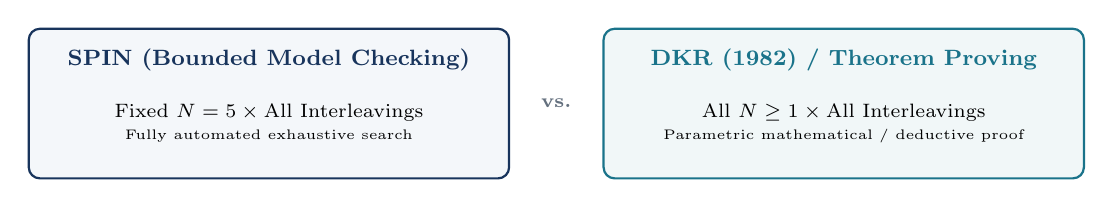
\begin{tikzpicture}
      \draw[draw=spinNavy, thick, fill=spinLight, rounded corners=4pt] (0.0,-0.95) rectangle (6.1,0.95);
      \node[font=\footnotesize\bfseries, text=spinNavy] at (3.05,0.55) {SPIN (Bounded Model Checking)};
      \node[font=\scriptsize, align=center] at (3.05,-0.25) {Fixed $N = 5 \times \text{All Interleavings}$\\{\tiny Fully automated exhaustive search}};

      \node[font=\scriptsize\bfseries, text=spinGray] at (6.70,0.0) {vs.};

      \draw[draw=spinTeal, thick, fill=spinTeal!6, rounded corners=4pt] (7.3,-0.95) rectangle (13.4,0.95);
      \node[font=\footnotesize\bfseries, text=spinTeal] at (10.35,0.55) {DKR (1982) / Theorem Proving};
      \node[font=\scriptsize, align=center] at (10.35,-0.25) {All $N \ge 1 \times \text{All Interleavings}$\\{\tiny Parametric mathematical / deductive proof}};
    \end{tikzpicture}
  \end{center}
  \note{2.0 min: Clarify scope of bounded model checking vs general mathematical proof.}
\end{frame}

% ==============================================================================
\section{Comparison \& Conclusions}
% ==============================================================================

% Frame 12 (~2.0 min)
\begin{frame}{Model Checking (SPIN) vs.\ Theorem Proving (Lean)}
  \small
  \renewcommand{\arraystretch}{1.35}
  \begin{tabular}{@{}L{0.20\textwidth}L{0.365\textwidth}L{0.365\textwidth}@{}}
    \toprule
    \rowcolor{spinNavy!10}
    \textbf{Dimension} & \textbf{SPIN (Model Checking)} & \textbf{Lean (Theorem Proving)} \\
    \midrule
    \textbf{User provides} & Bounded system model (PROMELA) + properties (LTL / assertions). & Formal definitions + theorem statements + logical proofs. \\
    \textbf{Verification \& feedback} & Automated exhaustive state-space search; outputs concrete counterexample traces. & Proof construction (with tactic automation) checked by a small kernel; outputs proof goals. \\
    \textbf{Guarantee scope} & Exhaustive for a fixed configuration (e.g., $N = 5$), under model assumptions. & Can establish parametric results for arbitrary $N$, at higher manual proof effort. \\
    \bottomrule
  \end{tabular}
  \vspace{0.7em}
  \begin{center}
    
\begin{tikzpicture}
      \node[draw=spinNavy!40, fill=spinLight, rounded corners=4pt, text width=13.2cm,
            align=center, inner sep=6pt, font=\footnotesize]
        {\textcolor{spinNavy}{\textbf{Takeaway:}} Complementary strengths --- SPIN excels at rapid automated bug finding in bounded designs; Lean excels at parametric proofs for arbitrary $N$.};
    \end{tikzpicture}
  \end{center}
  \note{2.0 min: Concise comparison in main deck; backup slide covers inductive invariants in detail.}
\end{frame}

% Frame 13 (~1.5 min)
\begin{frame}{Conclusions}
  \begin{itemize}
    \item \textbf{Design Methodology Supported by SPIN (Sec.\ 5):}
    \begin{enumerate}
      \item Separate \textbf{behavior} (PROMELA prototype) from \textbf{requirements} (LTL / assertions).
      \item Mechanically check internal and mutual consistency using \textbf{SPIN}.
      \item Revise the design until critical properties are verified \emph{before} full implementation.
    \end{enumerate}
  \end{itemize}
  \vspace{0.45em}
  \begin{center}
    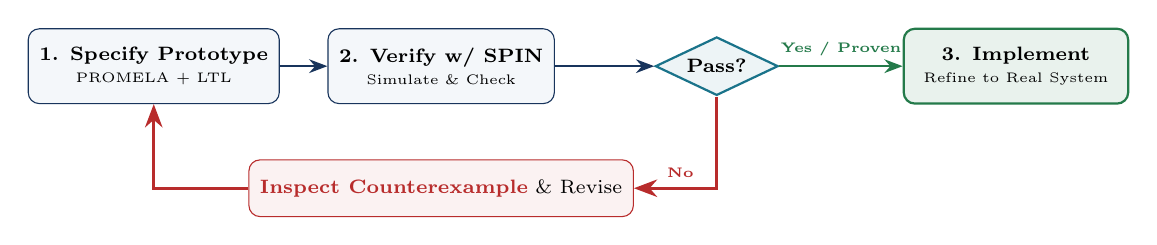
\begin{tikzpicture}[
      bx/.style={draw=spinNavy, fill=spinLight, rounded corners=4pt, font=\scriptsize,
                 minimum width=2.85cm, minimum height=0.95cm, align=center, inner sep=4pt},
      dia/.style={diamond, draw=spinTeal, thick, fill=spinTeal!8, aspect=2.1,
                  font=\scriptsize\bfseries, inner sep=2pt, align=center},
      arr/.style={->, >=Stealth, thick, color=spinNavy}
    ]
      \node[bx] (s1) at (0,0) {\textbf{1. Specify Prototype}\\{\tiny PROMELA + LTL}};
      \node[bx] (s2) at (3.65,0) {\textbf{2. Verify w/ SPIN}\\{\tiny Simulate \& Check}};
      \node[dia] (dec) at (7.15,0) {Pass?};
      \node[bx, draw=spinGreen, thick, fill=spinGreen!10] (s3) at (10.95,0) {\textbf{3. Implement}\\{\tiny Refine to Real System}};

      \draw[arr] (s1) -- (s2);
      \draw[arr] (s2) -- (dec);
      \draw[->, >=Stealth, thick, color=spinGreen] (dec) -- node[above, font=\tiny\bfseries, text=spinGreen] {Yes / Proven} (s3);

      % Red revision loop
      \node[bx, draw=spinRed, fill=spinRed!6, minimum width=3.1cm, minimum height=0.72cm] (rev) at (3.65,-1.55)
        {\textcolor{spinRed}{\textbf{Inspect Counterexample}} \& Revise};
      \draw[->, >=Stealth, very thick, color=spinRed] (dec.south) |- node[pos=0.72, above, font=\tiny\bfseries, text=spinRed] {No} (rev.east);
      \draw[->, >=Stealth, very thick, color=spinRed] (rev.west) -| (s1.south);
    \end{tikzpicture}
  \end{center}
  \note{1.5 min: Summarize Holzmann's engineering prototype workflow from Sec. 5.}
\end{frame}

% Frame 14: Dedicated Closing Q&A Slide (end of main deck: 14 / 14)
\begin{frame}[label=qa]{Questions \& Discussion}
  \vspace{1.2em}
  \begin{center}
    {\Huge\bfseries\textcolor{spinNavy}{Thank You!}}\\[0.8em]
    {\Large\textcolor{spinTeal}{Questions \& Discussion}}\\[1.4em]
    {\small\textcolor{spinGray}{Happy to discuss SPIN vs.\ Lean, modeling assumptions, or other case studies from Holzmann (1997).}}
  \end{center}
  \vspace{2.2em}
  \begin{center}
    \hyperlink{backup1}{\beamergotobutton{Backup 1: SPIN vs.\ Lean Invariant}}\quad
    \hyperlink{backup2}{\beamergotobutton{Backup 2: Other Case Studies}}\quad
    \hyperlink{backup3}{\beamergotobutton{Backup 3: LTL \& Negated Claims}}
  \end{center}
  \note{Remaining ~4.5 min for Q&A; buttons jump to Appendix Backup slides.}
\end{frame}

% ==============================================================================
\appendix
% ==============================================================================

% Frame 15 (Backup 1)
\begin{frame}[label=backup1]{Backup 1: Leader Election Safety in SPIN vs.\ Lean}
  \textbf{Target Safety Property:} ``At most one leader is ever elected'' ($\text{nr\_leaders} \le 1$).
  \vspace{0.5em}
  \begin{columns}[T]
    \begin{column}{0.48\textwidth}
      \begin{block}{In SPIN (Model Checking)}
        \begin{itemize}
          \item Fix bounded parameters ($N = 5$, $L = 10$).
          \item Encode process transitions in PROMELA.
          \item SPIN automatically explores all reachable states and verifies $\text{nr\_leaders} \le 1$ (or returns a trace on failure).
        \end{itemize}
      \end{block}
    \end{column}
    \begin{column}{0.48\textwidth}
      \begin{block}{In Lean (Deductive Theorem Proving)}
        \begin{itemize}
          \item Discover and prove an \textbf{inductive invariant} $I(s)$:
          \begin{enumerate}
            \item \textbf{Initiation:} $I(s_0)$ holds initially.
            \item \textbf{Preservation:} $s \to s' \implies (I(s) \implies I(s'))$.
            \item \textbf{Safety:} $I(s) \implies \text{nr\_leaders}(s) \le 1$.
          \end{enumerate}
          \item Proves safety for \textbf{arbitrary $N$}, at manual proof cost.
        \end{itemize}
      \end{block}
    \end{column}
  \end{columns}
  \vspace{1.0em}
  \hfill\hyperlink{qa}{\beamergotobutton{Back to Q\&A}}
  \note{Backup 1: Concrete comparison on safety invariant vs bounded search.}
\end{frame}

% Frame 16 (Backup 2)
\begin{frame}[label=backup2]{Backup 2: Other Case Studies in Holzmann (1997)}
  \begin{block}{Process Scheduling (Sec.\ 4.1, UTS Kernel Sleep/Wakeup)}
    \begin{itemize}
      \item Two asynchronous processes (\texttt{client}, \texttt{server}) share spinlock \texttt{lk} and resource flag \texttt{r\_lock}.
      \item SPIN catches the lost-wakeup non-progress cycle \emph{and} proves the designer's proposed fix still fails; the real fix reclaims \texttt{lk} via \texttt{goto sleep}.
    \end{itemize}
  \end{block}
  \vspace{0.3em}
  \begin{block}{Go-Back-N Sliding Window Protocol (Sec.\ 4.3, Tanenbaum)}
    \begin{itemize}
      \item XSPIN message-sequence simulation catches a sequence-number increment error (\texttt{MaxSeq} vs.\ \texttt{MaxSeq + 1}).
      \item Faithful delivery (liveness) verified via Wolper's 3-color (\texttt{red}/\texttt{white}/\texttt{blue}) data-independence reduction.
    \end{itemize}
  \end{block}
  \vspace{0.5em}
  \hfill\hyperlink{qa}{\beamergotobutton{Back to Q\&A}}
  \note{Backup 2: Ready if audience asks about Sec. 4.1 or 4.3.}
\end{frame}

% Frame 17 (Backup 3)
\begin{frame}[label=backup3]{Backup 3: LTL Operators \& Why Negated Claims? (Sec.\ 2.1)}
  \begin{columns}[T]
    \begin{column}{0.48\textwidth}
      \begin{block}{Core LTL Grammar (Fig.\ 2)}
        \begin{itemize}
          \item \texttt{[]} $p$: always $p$ (safety / invariance).
          \item \texttt{<>} $p$: eventually $p$ (liveness).
          \item $p$ \texttt{U} $q$: $p$ holds strong-until $q$ becomes true.
          \item Boolean: \texttt{!}, \texttt{\&\&}, \texttt{||}, \texttt{->}, \texttt{<->}.
        \end{itemize}
      \end{block}
    \end{column}
    \begin{column}{0.48\textwidth}
      \begin{block}{Positive vs.\ Negative Claims (Sec.\ 2.1)}
        \begin{itemize}
          \item Positive claim $L(S) \subseteq L(\varphi)$: product size is at least $|S| + |C|$.
          \item Negative claim $L(S) \cap L(\neg\varphi) = \emptyset$: worst-case $|S| \times |C|$, \textbf{best-case $0$ states} if no bad prefix exists in $S$.
        \end{itemize}
      \end{block}
    \end{column}
  \end{columns}
  \vspace{1.2em}
  \hfill\hyperlink{qa}{\beamergotobutton{Back to Q\&A}}
  \note{Backup 3: Ready if audience asks about LTL syntax or automata emptiness check.}
\end{frame}

\end{document}
